\documentclass{beamer}
\usepackage[T1]{fontenc}
\usepackage[utf8]{inputenc}
\usepackage{graphicx}
\usepackage[normalem]{ulem}
\usepackage{xmpmulti}
\usepackage{marvosym}
% \usepackage[dvipsnames]{xcolor}
% \usepackage{enumitem}


\newcommand{\emphh}[1]{\textcolor{blue}{\emph{#1}}}
\newcommand{\hilite}[1]{\emphh{#1}}
\title{Erdős-Pósa for Pairwise Distant Cycles}

\newcommand{\verteq}{\rotatebox{90}{$\equiv$}}

\author{}
\author{%
  Vida~Dujmović \and
  Gwenaël~Joret \and
  Piotr~Micek \and
  Pat Morin \\[3ex]
  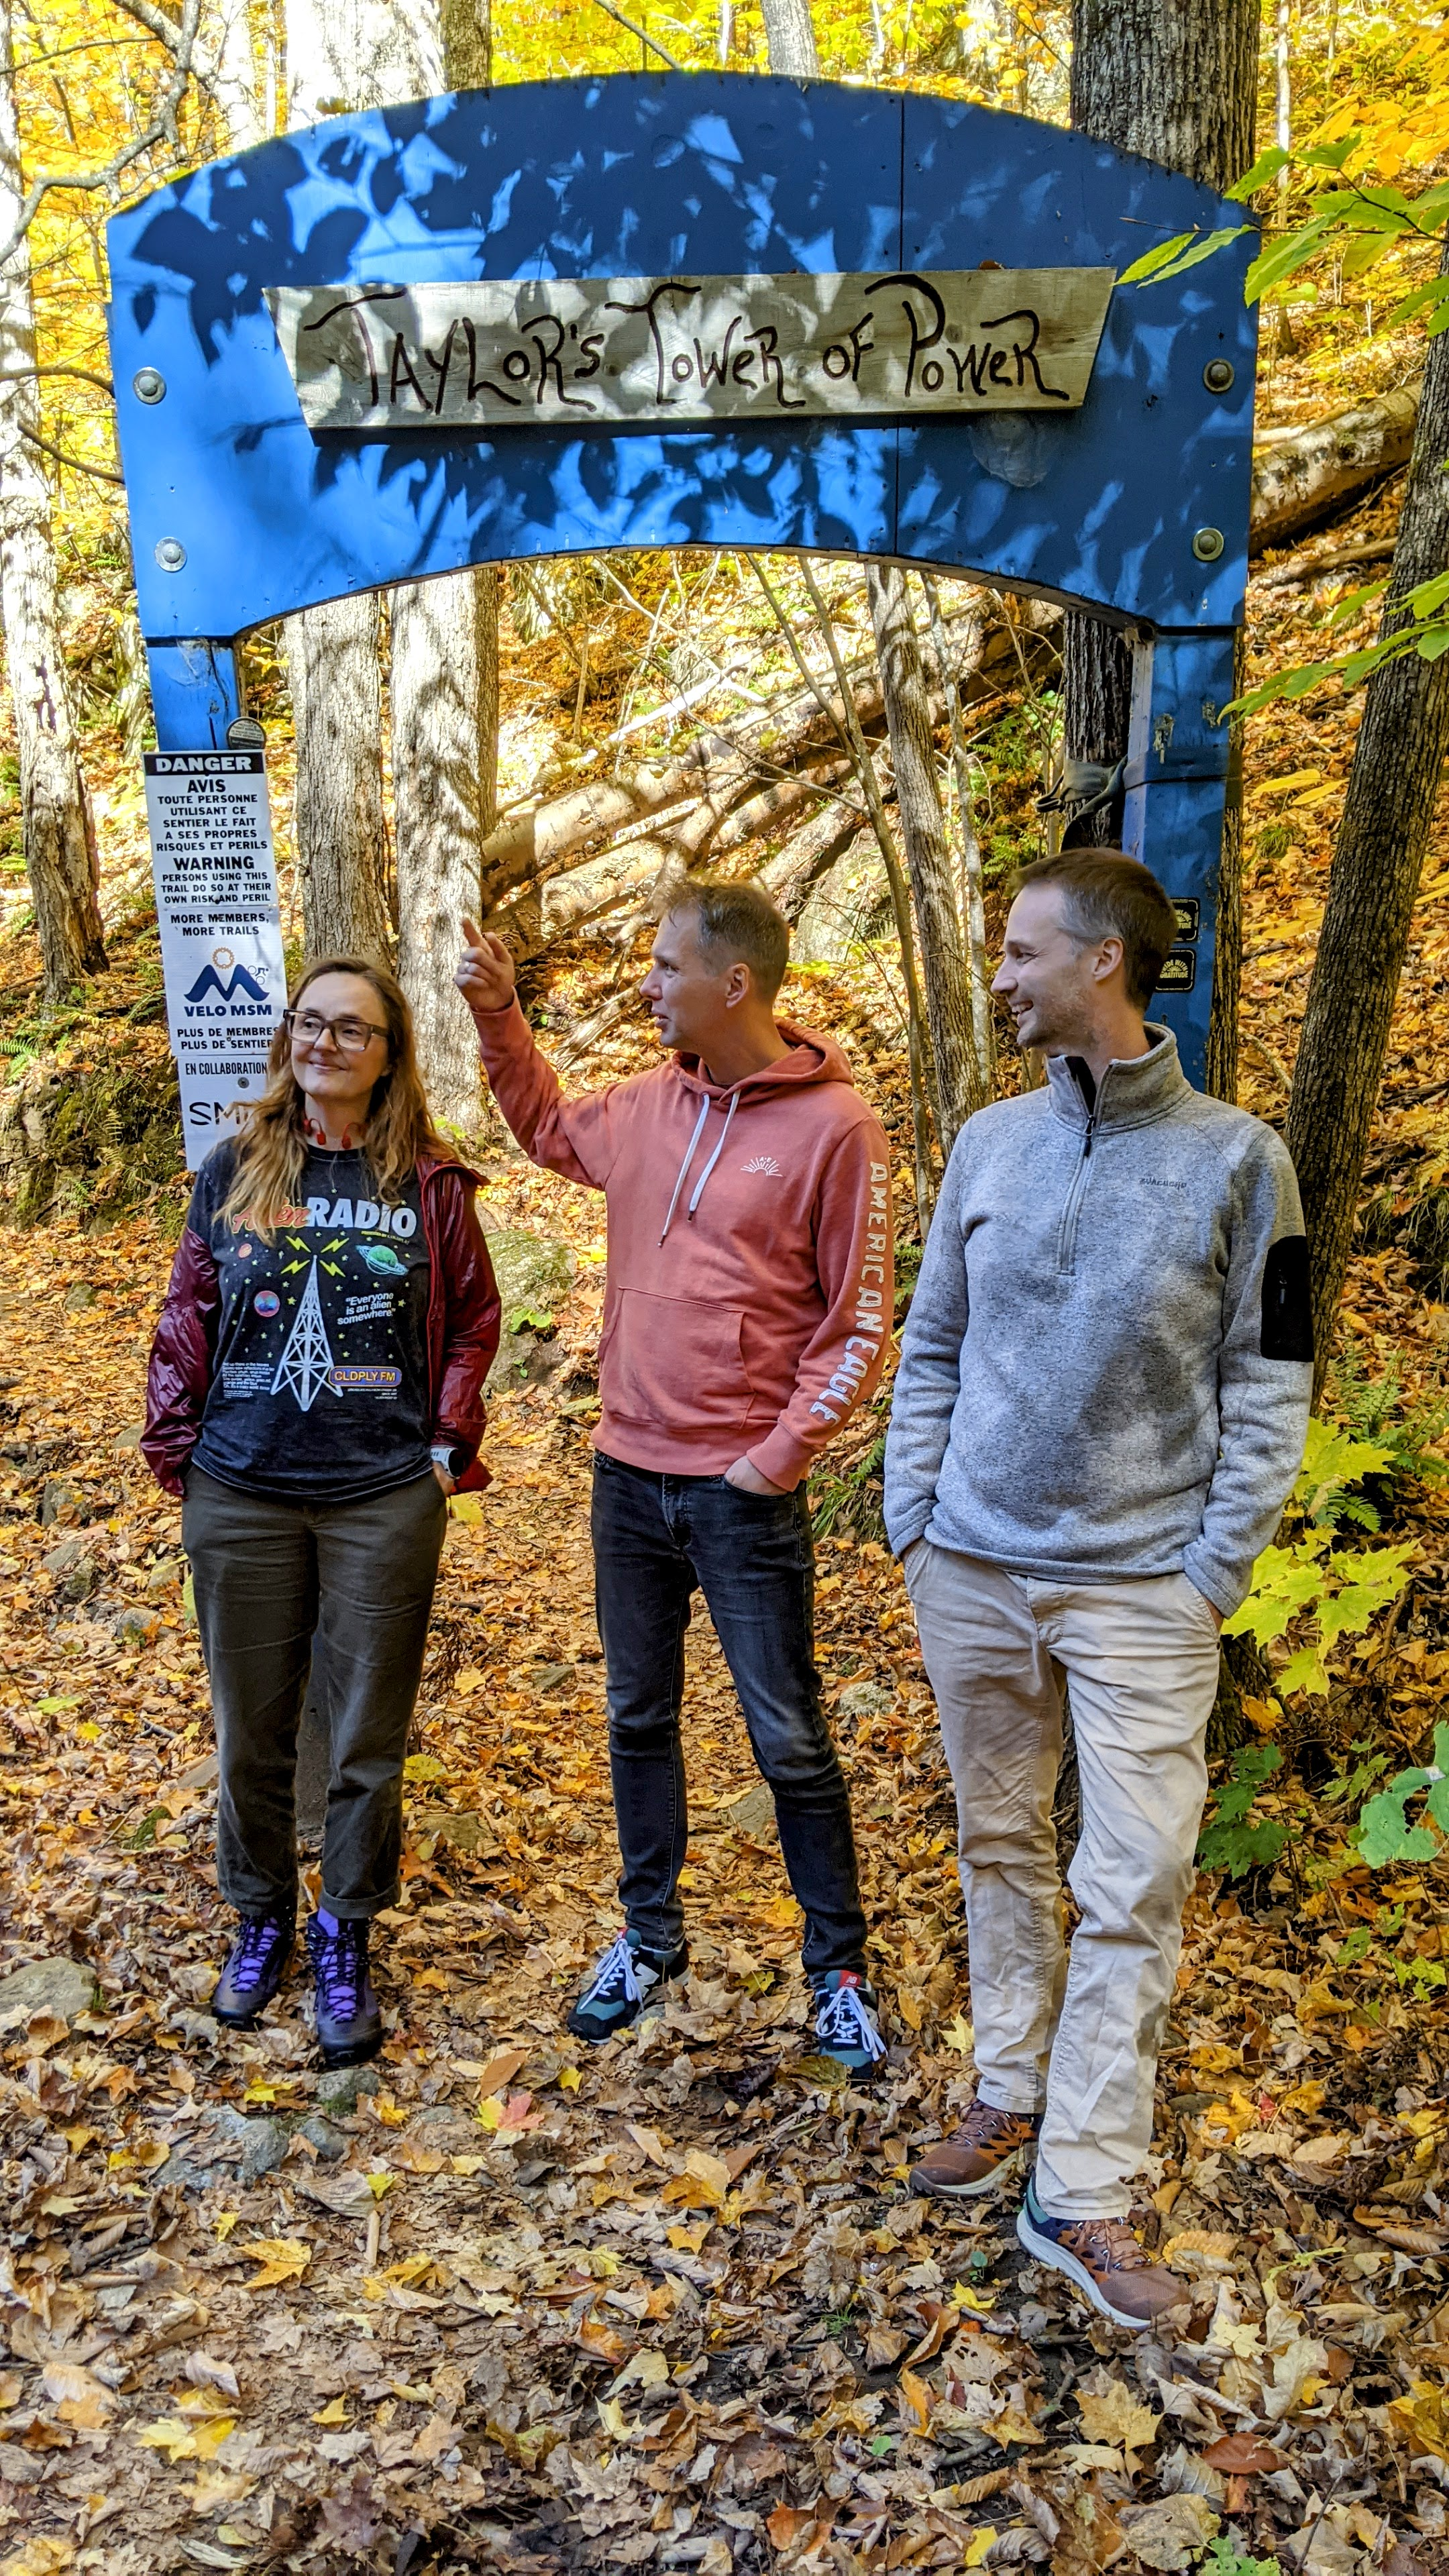
\includegraphics[height=.4\textheight]{images/ttop-hdr}
  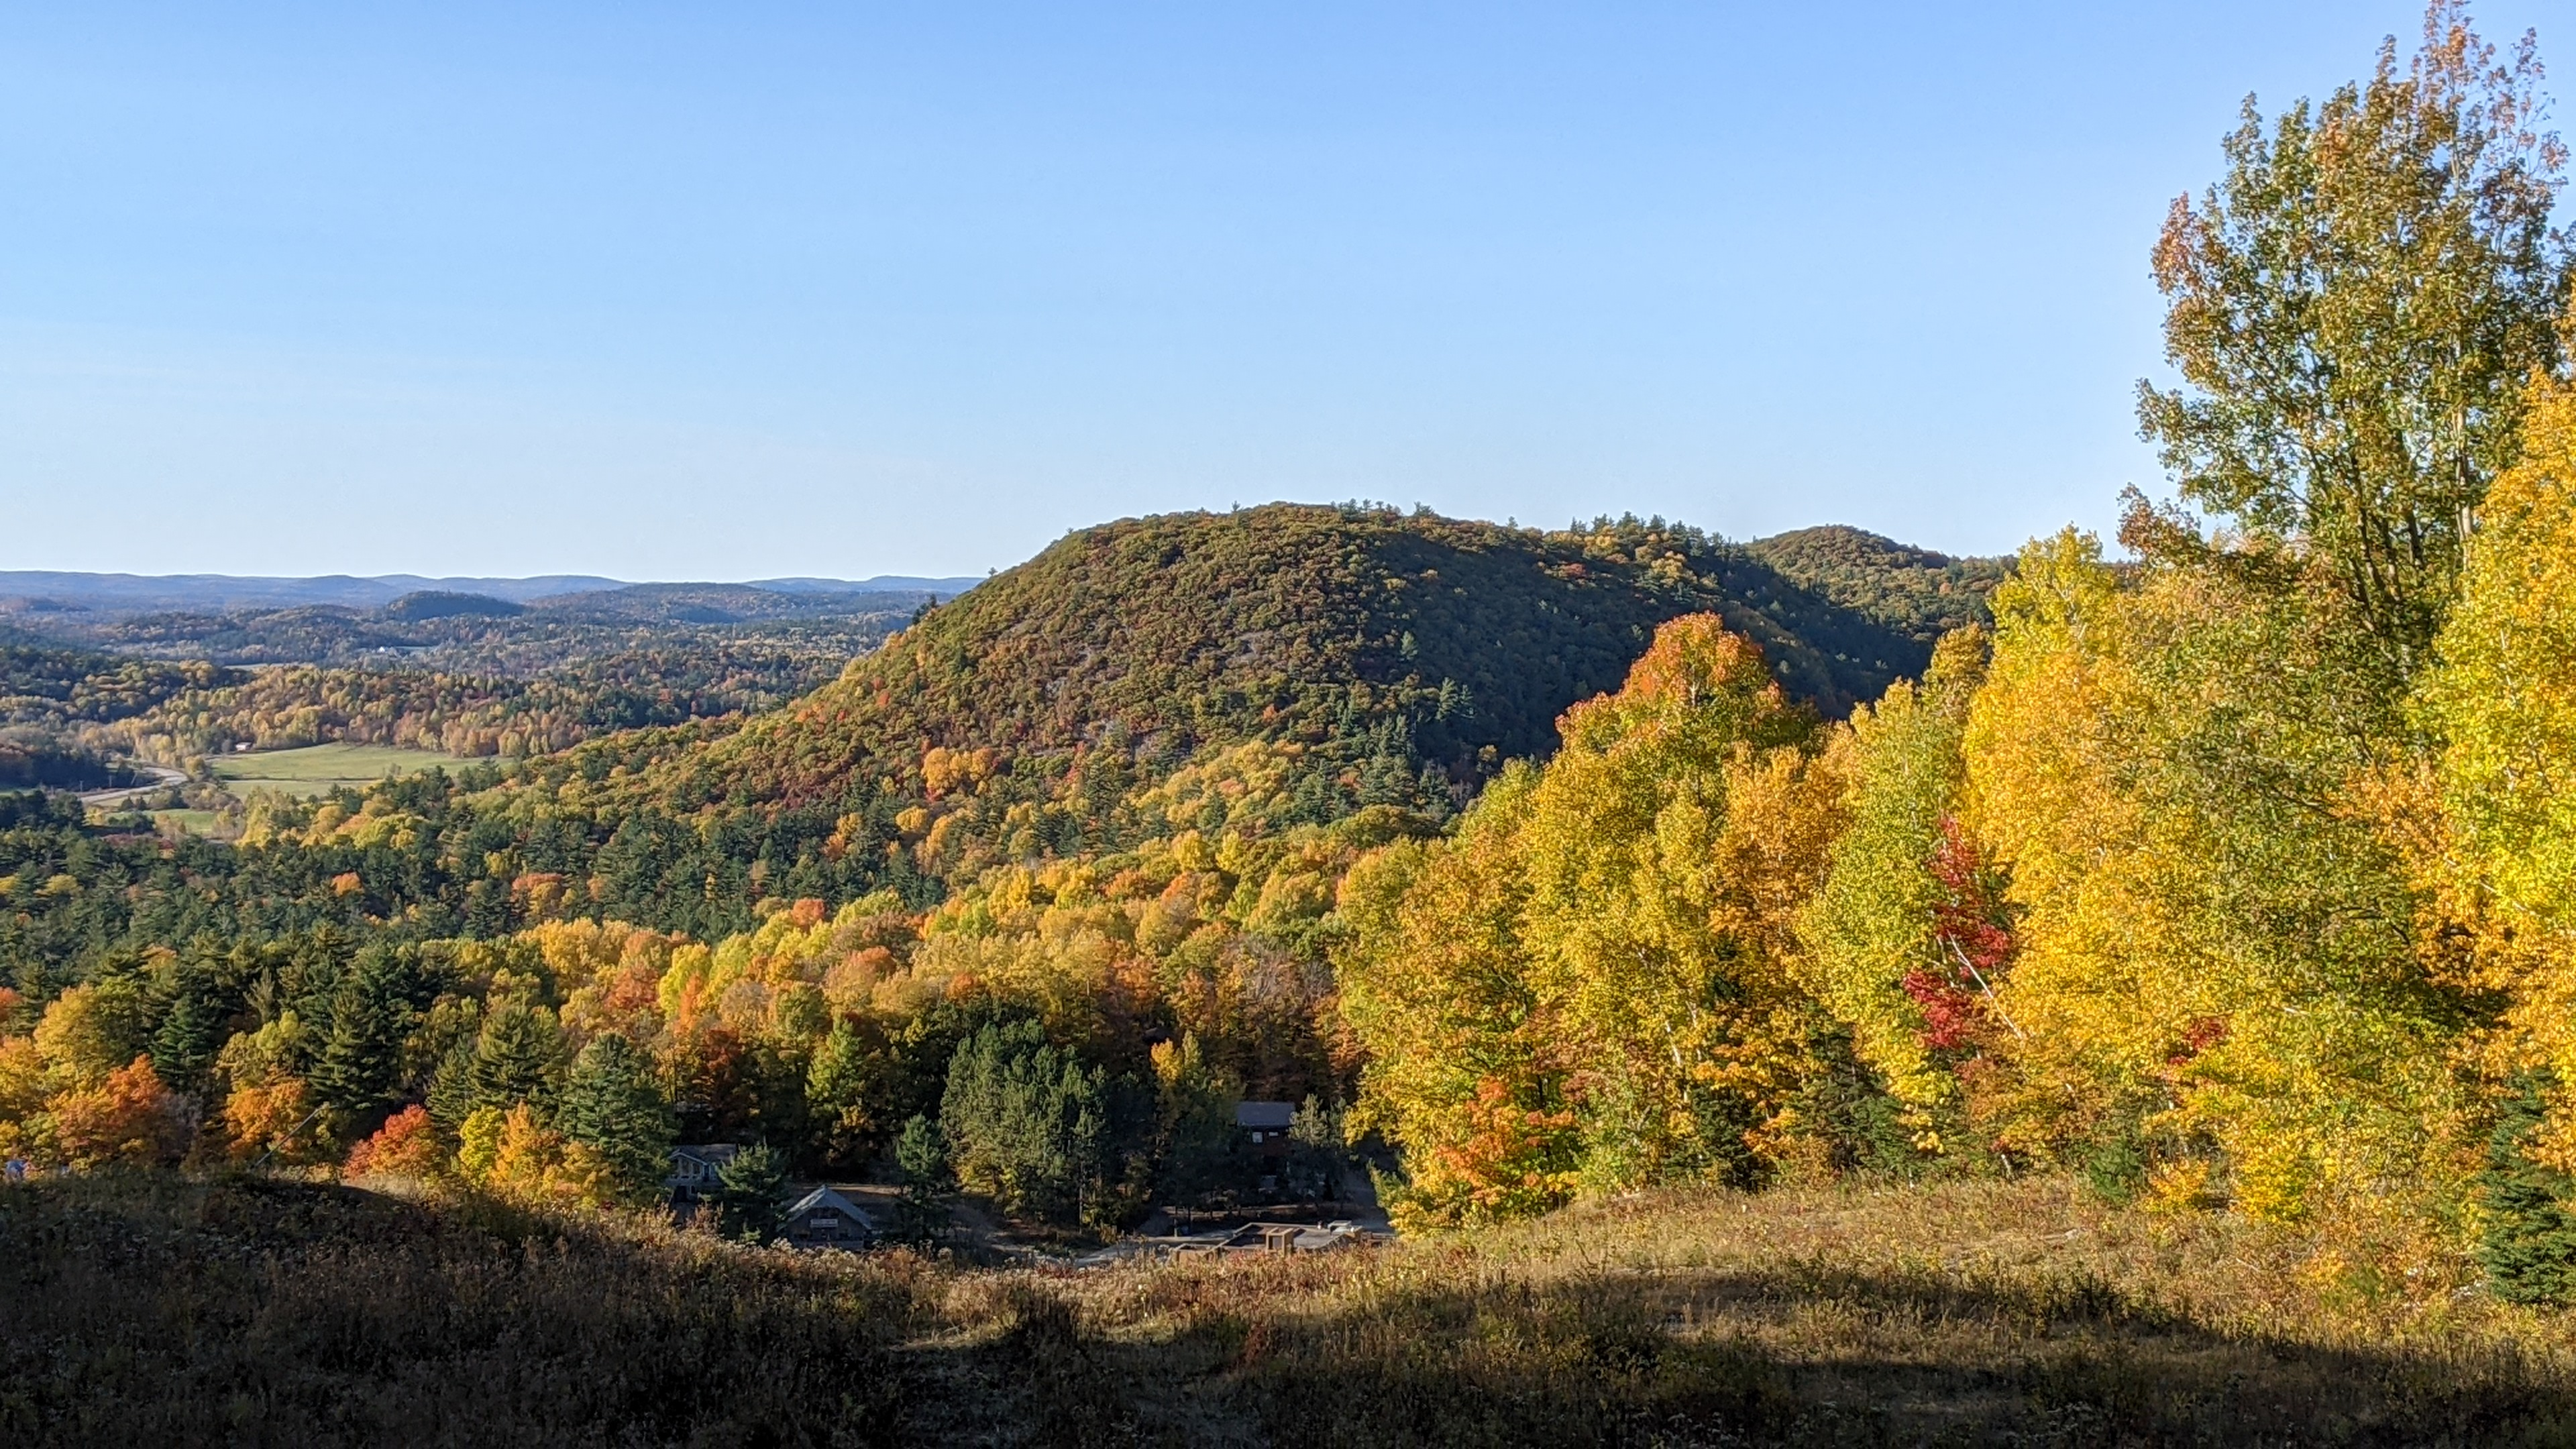
\includegraphics[height=.4\textheight]{images/view}}
\date{}

\setbeameroption{hide notes} % Only slides
%\setbeameroption{show only notes} % Only notes
% \setbeameroption{show notes on second screen=right} % Both


% \DeclareMathOperator{\tw}{tw}
% \DeclareMathOperator{\td}{td}
% \DeclareMathOperator{\wcol}{wcol}
% \DeclareMathOperator{\lvr}{\chi_{\ell-\mathrm{vr}}}
% \DeclareMathOperator{\pcn}{\chi_{p}}
\newcommand{\N}{\mathbb{N}}
\begin{document}

\begin{frame}
  % \begin{center}
    \maketitle
  % \end{center}
\end{frame}

\begin{frame}
  \frametitle{Outline}

  \begin{itemize}
    \item Theorem statement
    \item Some related work
    \item Proof sketch
  \end{itemize}
\end{frame}


\begin{frame}
  \frametitle{Main Theorem}

  \noindent\textbf{Theorem (Dujmović-Joret-Micek-M 2024):} There exists functions $f,g:\N\to\N$ such that, for every graph $G$, every integer $k\ge 1$ and every integer $d\ge 0$,
  \begin{enumerate}%[nosep,nolistsep]
    \item $G$ contains \textcolor{blue}{$d$-packing} of $k$ cycles \textbf{or}
    \item $G$ has a vertex subset $\mathcolor{red}{X}$ of size at most $f(k)$ such that $G-B(X,g(d))$ is a forest.  \newline \uncover<2->{(Every cycle in $G$ contains a vertex in $\mathcolor{blue}{B(X, g(d))}$.)}
  \end{enumerate}

  \begin{center}
    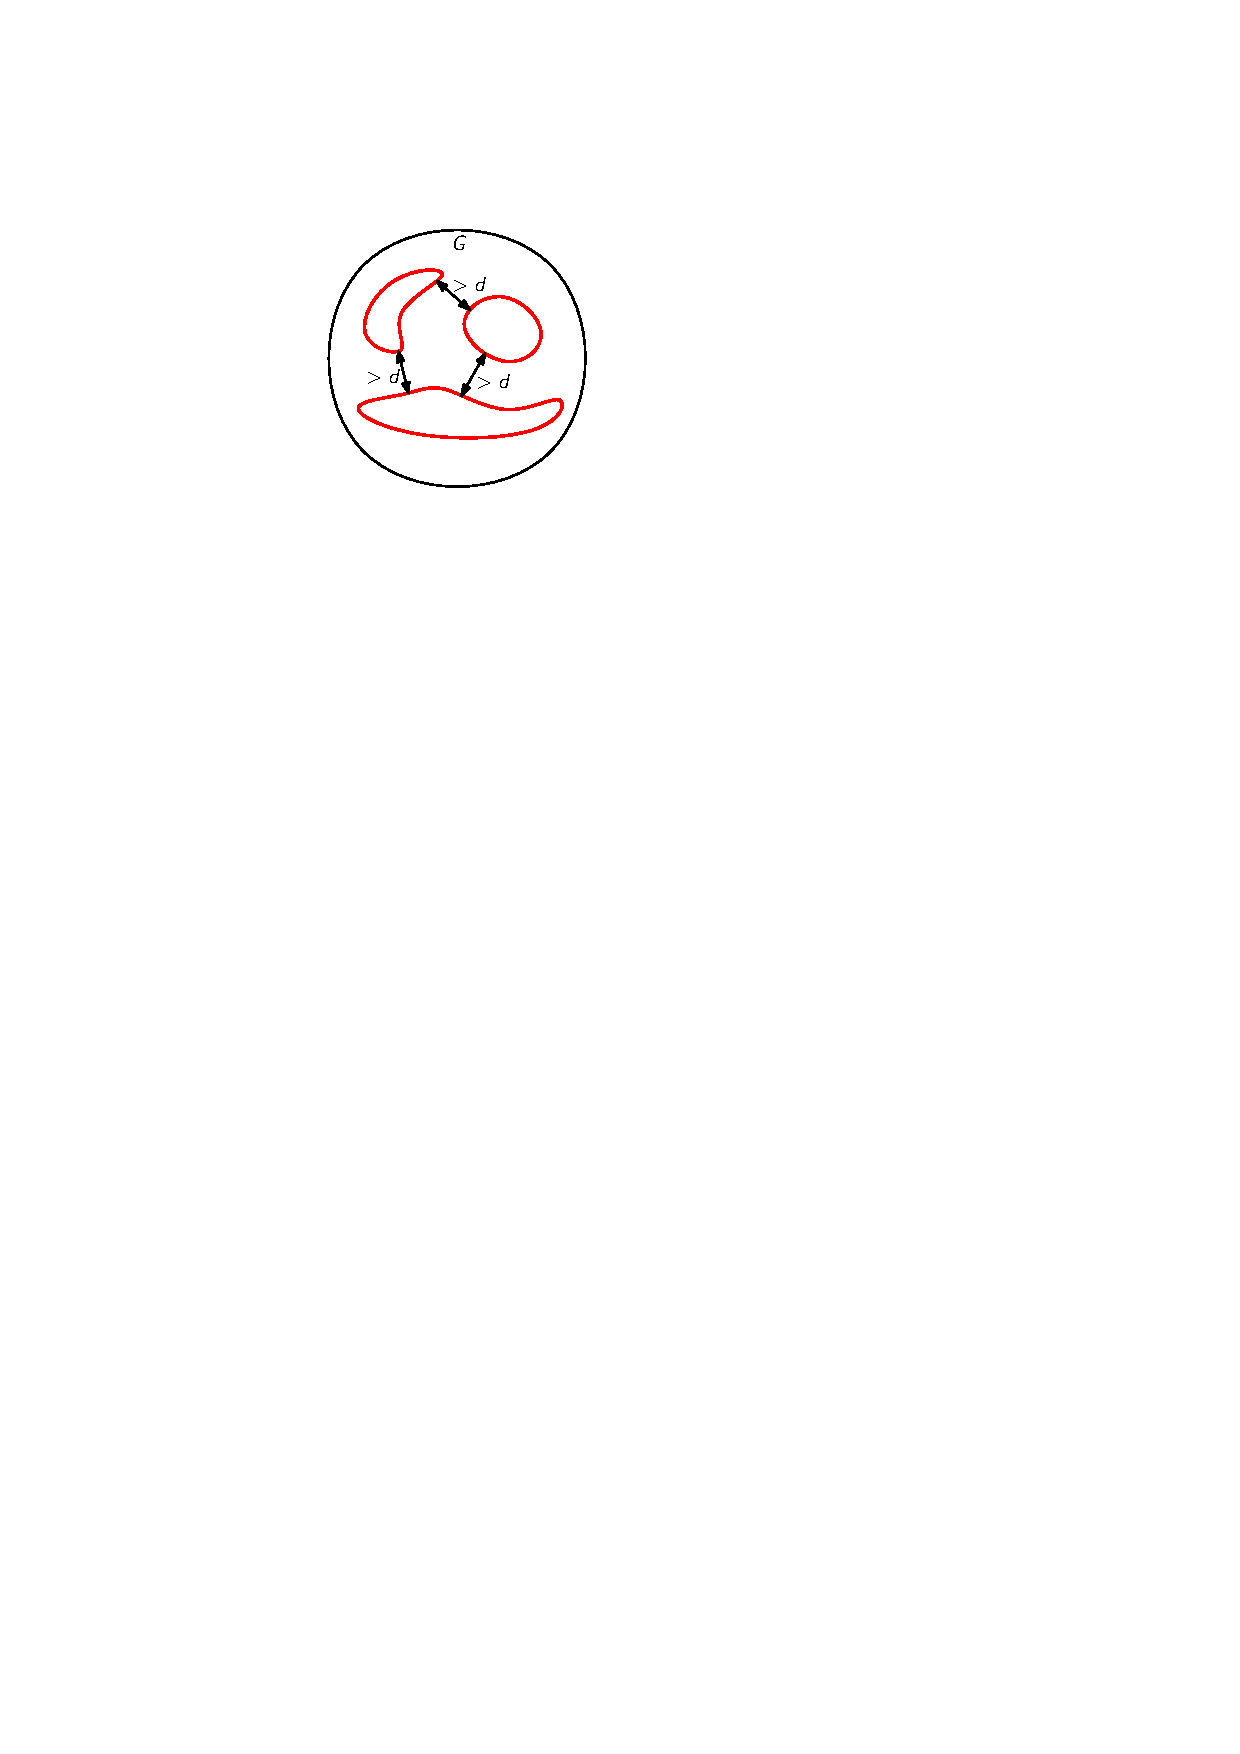
\includegraphics[scale=.9,page=1]{figs/cep}
    \raisebox{2cm}{ OR }
    \includegraphics[scale=.9,page=2]{figs/cep}
  \end{center}
  \uncover<3->{(And $f(k)\in O((k\log k)^{18})$ and $g(d)\le 19d$.)}
\end{frame}


\begin{frame}
  \frametitle{$d=0$: The Erdős-Pósa Theorem}

    \noindent\textbf{Theorem (Erdős-Pósa 1965):}
    For every graph $G$ and every integer $k\ge 1$,
    \begin{enumerate}%[nosep,nolistsep]
      \item[(a)] $G$ contains $k$ pairwise vertex-disjoint cycles \textbf{or}
      \item[(b)] $G$ has a vertex subset $\mathcolor{red}{X}$ of size $O(k\log k)$ such that $G-X$ is a forest. \uncover<3>{\textcolor{blue}{(Every cycle in $G$ has a vertex in $X$.)}}
    \end{enumerate}
    \begin{center}
      \only<1>{\includegraphics[page=3]{figs/erdos_posa}}%
      \only<2->{\includegraphics[page=4]{figs/erdos_posa}}
      \uncover<2->{\raisebox{2cm}{ OR }}
      \only<1>{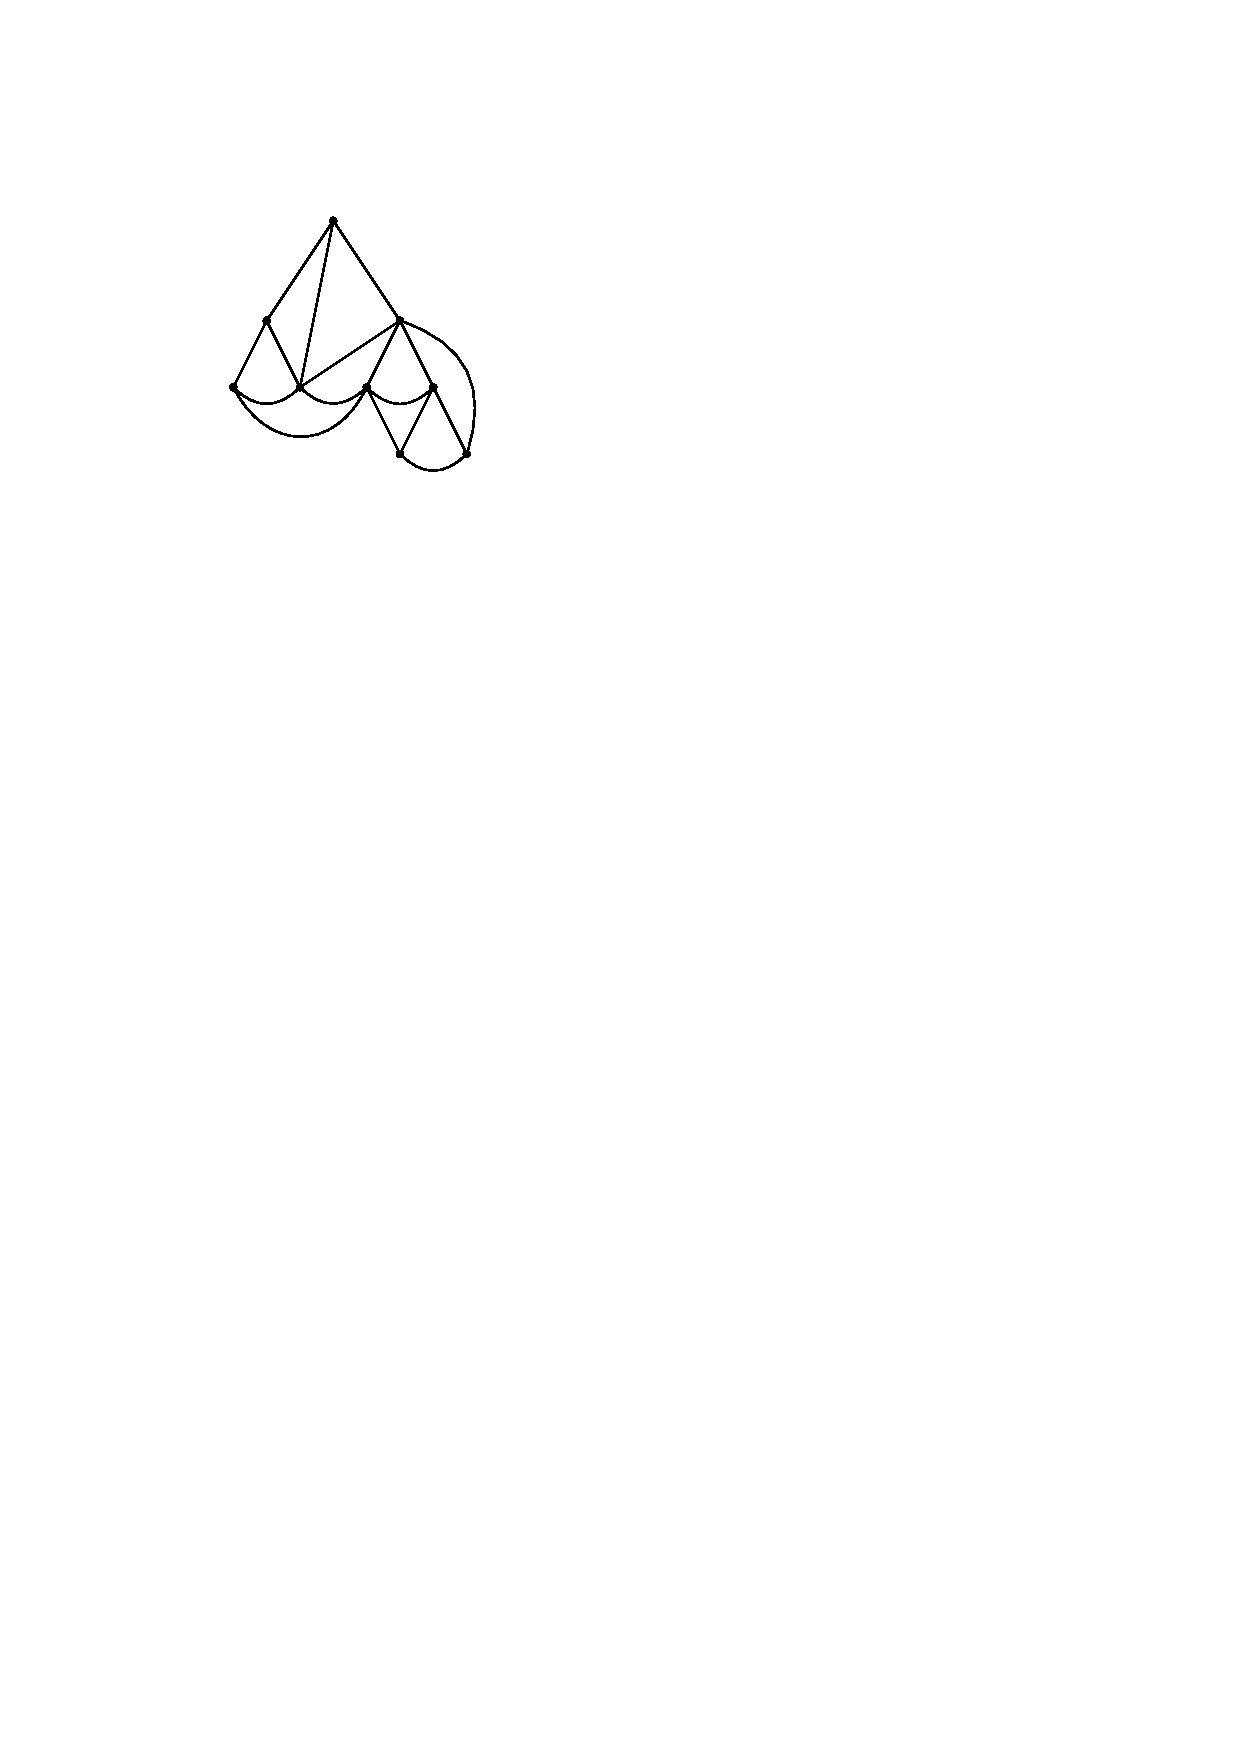
\includegraphics[page=1]{figs/erdos_posa}}%
      \only<2->{\includegraphics[page=2]{figs/erdos_posa}}
    \end{center}
\end{frame}

\begin{frame}
  \frametitle{$d=1$ and $k=2$}


  \noindent\textbf{Theorem (Ahn-Gollin-Huynh-Kwon 2024):} For every graph $G$ and every integer $k\ge 1$,
  \begin{enumerate}%[nosep,nolistsep]
    \item[(a)] $G$ contains an \textcolor{blue}{induced packing} of $k$ cycles \textbf{or}
    \item[(b)] $G$ has a vertex subset $\mathcolor{red}{X}$ of size $f(k)$ such that $G-B(X,1)$ is a forest.
  \end{enumerate}
  \ \\[2ex]
  \noindent\textbf{Theorem (Ahn-Gollin-Huynh-Kwon 2024):} For every graph $G$ and every integer $d\ge 0$,
  \begin{enumerate}%[nosep,nolistsep]
    \item $G$ contains a pair of cycles at distance greater than $d$ \textbf{or}
    \item $G$ has a vertex subset $\mathcolor{red}{X}$ of size at most $12(d+2)$ such that $G-B(X,3d)$ is a forest.
  \end{enumerate}
\end{frame}


\begin{frame}
  \frametitle{A Robertson-Seymour Erdős-Pósa-Type Theorem}
  \framesubtitle{An Application of the Grid-Minor Theorem}

  \noindent\textbf{Theorem (Robertson-Seymour 1986):} For every graph $G$, every integer $k\ge 1$,  and every planar graph $H$,
  \begin{enumerate}%[nosep,nolistsep]
    \item[(a)] $G$ contains $k$ pairwise vertex-disjoint $H$ minors \textbf{or}
    \item[(b)] $G$ has a vertex subset $\mathcolor{red}{X}$ of size at most $f(H)$ such that $G-X$ is $H$-minor-free. \textcolor{blue}{(Every model of $H$ in $G$ has a vertex in $X$.)}
  \end{enumerate}
  \ \\[3ex]
  (Really a statement about bounded treewidth graphs $G$)
\end{frame}


\begin{frame}
  \frametitle{An Erdős-Pósa-Type Theorem for Subtrees}

  \noindent{\textbf{Definition:} A \textcolor{blue}{subtree} in a tree $T$ is a subgraph of $T$ with $1$ component.\\[3ex]}

  \noindent\textbf{Theorem:} For every tree $T$, every integer $k\ge 1$,  and every collection $\mathcal{C}$ of subtrees of $T$,
  \begin{enumerate}%[nosep,nolistsep]
    \item[(a)] $\mathcal{C}$ contains $k$ pairwise vertex-disjoint subtrees \textbf{or}
    \item[(b)] $G$ has a vertex subset $\mathcolor{red}{X}$ of size at most $k-1$ such that every subtree in $\mathcal{C}$ contains a vertex in $X$.
  \end{enumerate}
  \ \\[3ex]
  (Establishes RS86 when $H$ is connected.)
\end{frame}


\begin{frame}
  \frametitle{An Erdős-Pósa-Type Theorem for $c$-Subtrees}

  \noindent{\textbf{Definition:} A \textcolor{blue}{$c$-subtree} in a forest $F$ is a non-empty subgraph of $F$ with at most $c$ components.\\[3ex]}

  \noindent\textbf{Theorem (Gyárfás-Lehel 1970):} For every forest $F$, every integer $k\ge 1$, and every collection $\mathcal{C}$ of $c$-subtrees of $F$,
  \begin{enumerate}%[nosep,nolistsep]
    \item[(a)] $\mathcal{C}$ contains $k$ pairwise vertex-disjoint $c$-subtrees \textbf{or}
    \item[(b)] $G$ has a vertex subset $\mathcolor{red}{X}$ of size at most $\ell^\star(k,c)$ such that every $c$-subtree in $\mathcal{C}$ contains a vertex in $X$.
  \end{enumerate}
  \ \\[3ex]
  (Establishes RS86 when $H$ has $c$ components.)
\end{frame}


\begin{frame}
  \frametitle{Simonovits' Theorem}

  \noindent\textbf{Theorem (Simonovits 1967):} Every (subdivision of every) cubic multigraph $G$ with at least $C k\log k$ vertices contains $k$ pairwise vertex-disjoint cycles.

  \only<1>{\includegraphics[scale=1.2,page=22,trim={1cm 2cm 2cm 0}]{figs/animation}}%
  \only<2>{\includegraphics[scale=1.2,page=21,trim={1cm 2cm 2cm 0}]{figs/animation}}
  \ \\[2ex]
  Helpful for establishing outcome (a) in Erd\H{o}s-Pósa Theorem
\end{frame}


\begin{frame}
  \frametitle{Main Theorem}

  \noindent\textbf{Theorem (Dujmović-Joret-Micek-M 2024):} For every graph $G$, every integer $k\ge 1$ and $d\ge 0$,
  \begin{enumerate}%[nosep,nolistsep]
    \item[(a)] $G$ contains \textcolor{blue}{$d$-packing} of $k$ cycles \textbf{or}
    \item[(b)] $G$ has a vertex subset $\mathcolor{red}{X}$ of size at most $f(k)$ such that every cycle in $G$ contains a vertex in $\mathcolor{blue}{B(X, g(d))}$.
  \end{enumerate}
  \begin{minipage}[t][.5\textheight]{\textwidth}
    \only<1>{%
      \begin{center}
        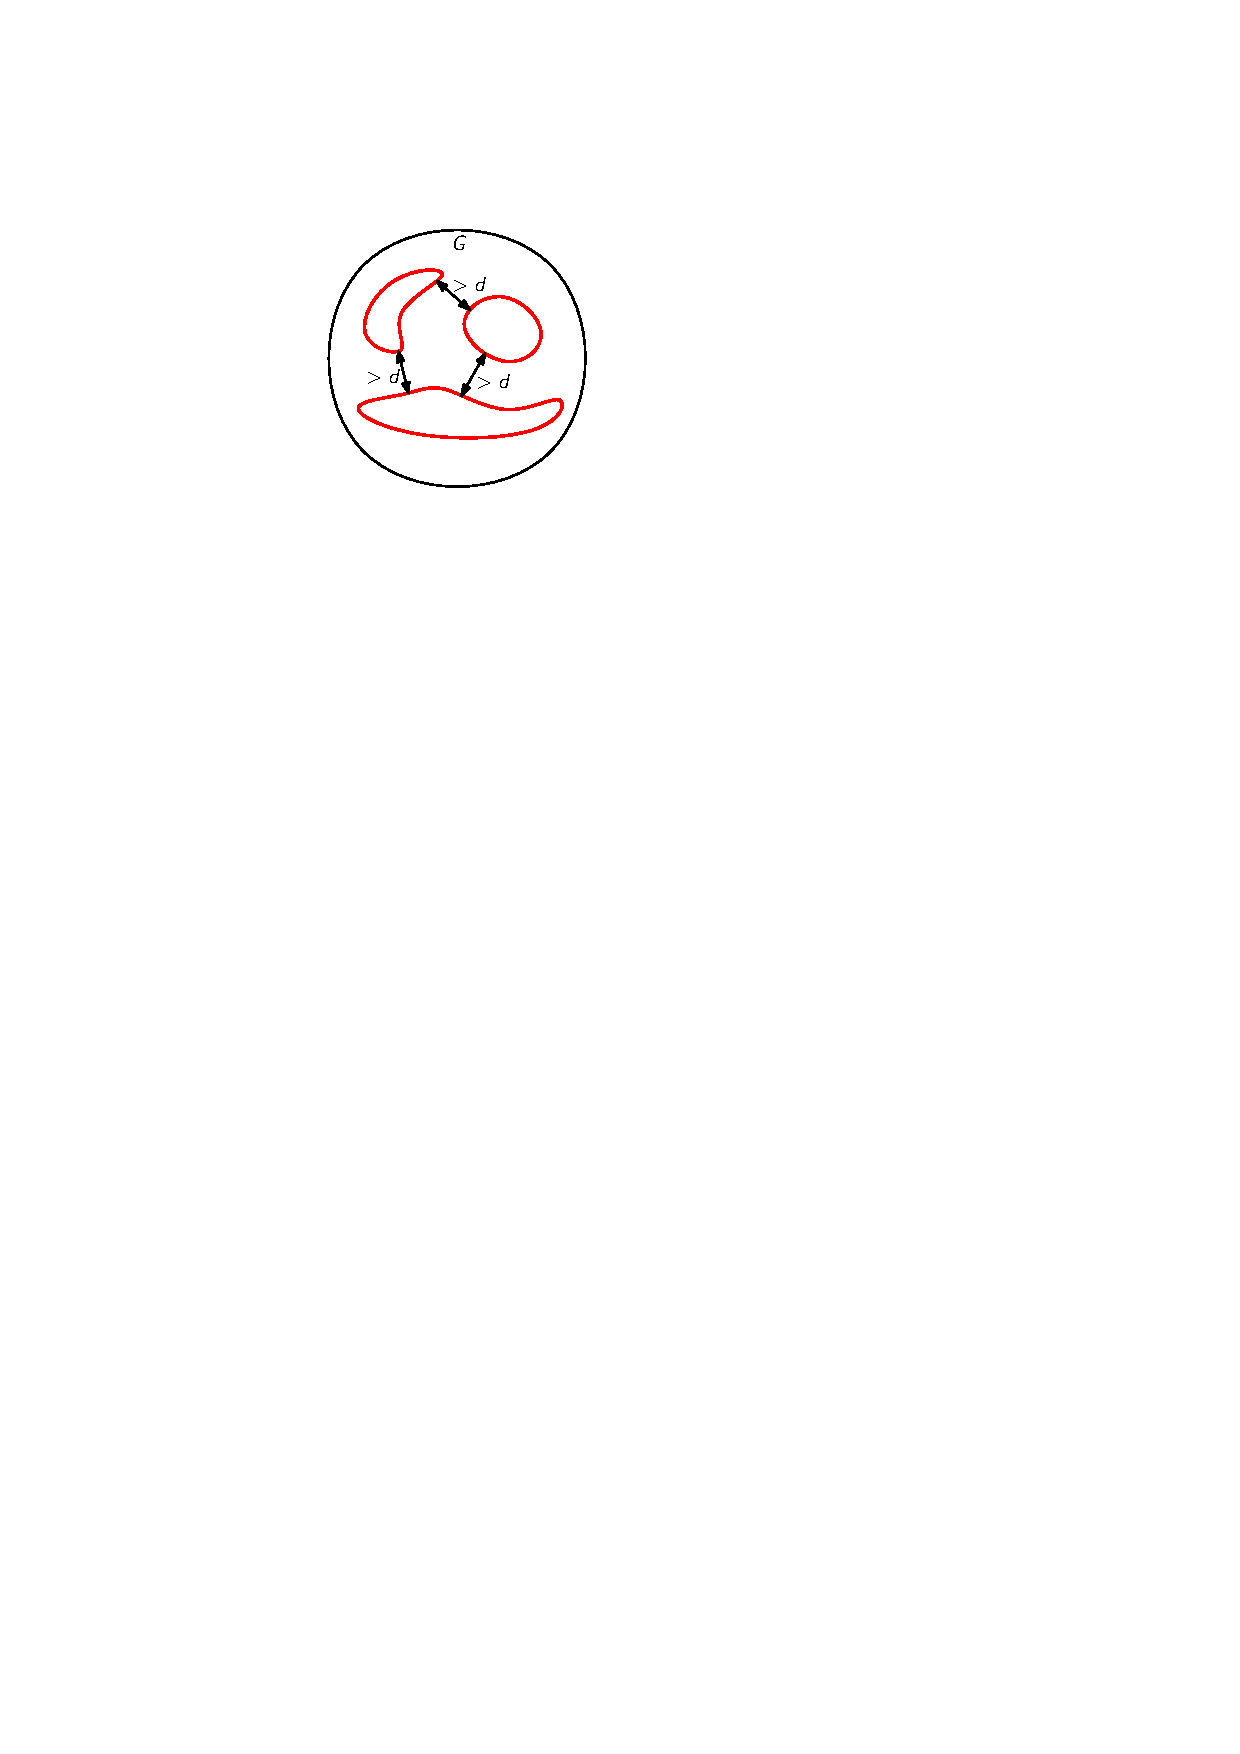
\includegraphics[page=1]{figs/cep}
        \raisebox{2cm}{ OR }
        \includegraphics[page=2]{figs/cep}
      \end{center}
    }%
    \only<2>{%
      \ \\[1ex]
      \emph{Proof:}
      \ \\[1ex]
      Assume $\neg{(\mathsf{a})}$: $G$ has no $d$-packing of $k$ cycles.\\[3ex]
      Prove (b): Construct $X\subseteq V(G)$, with $|X|\le f(k)$ such that every cycle in $G$ contains a vertex in $B(X,g(d))$
    }
    \end{minipage}
\end{frame}

\begin{frame}
  \frametitle{Proof Outline (in Pictures)}

  \only<1>{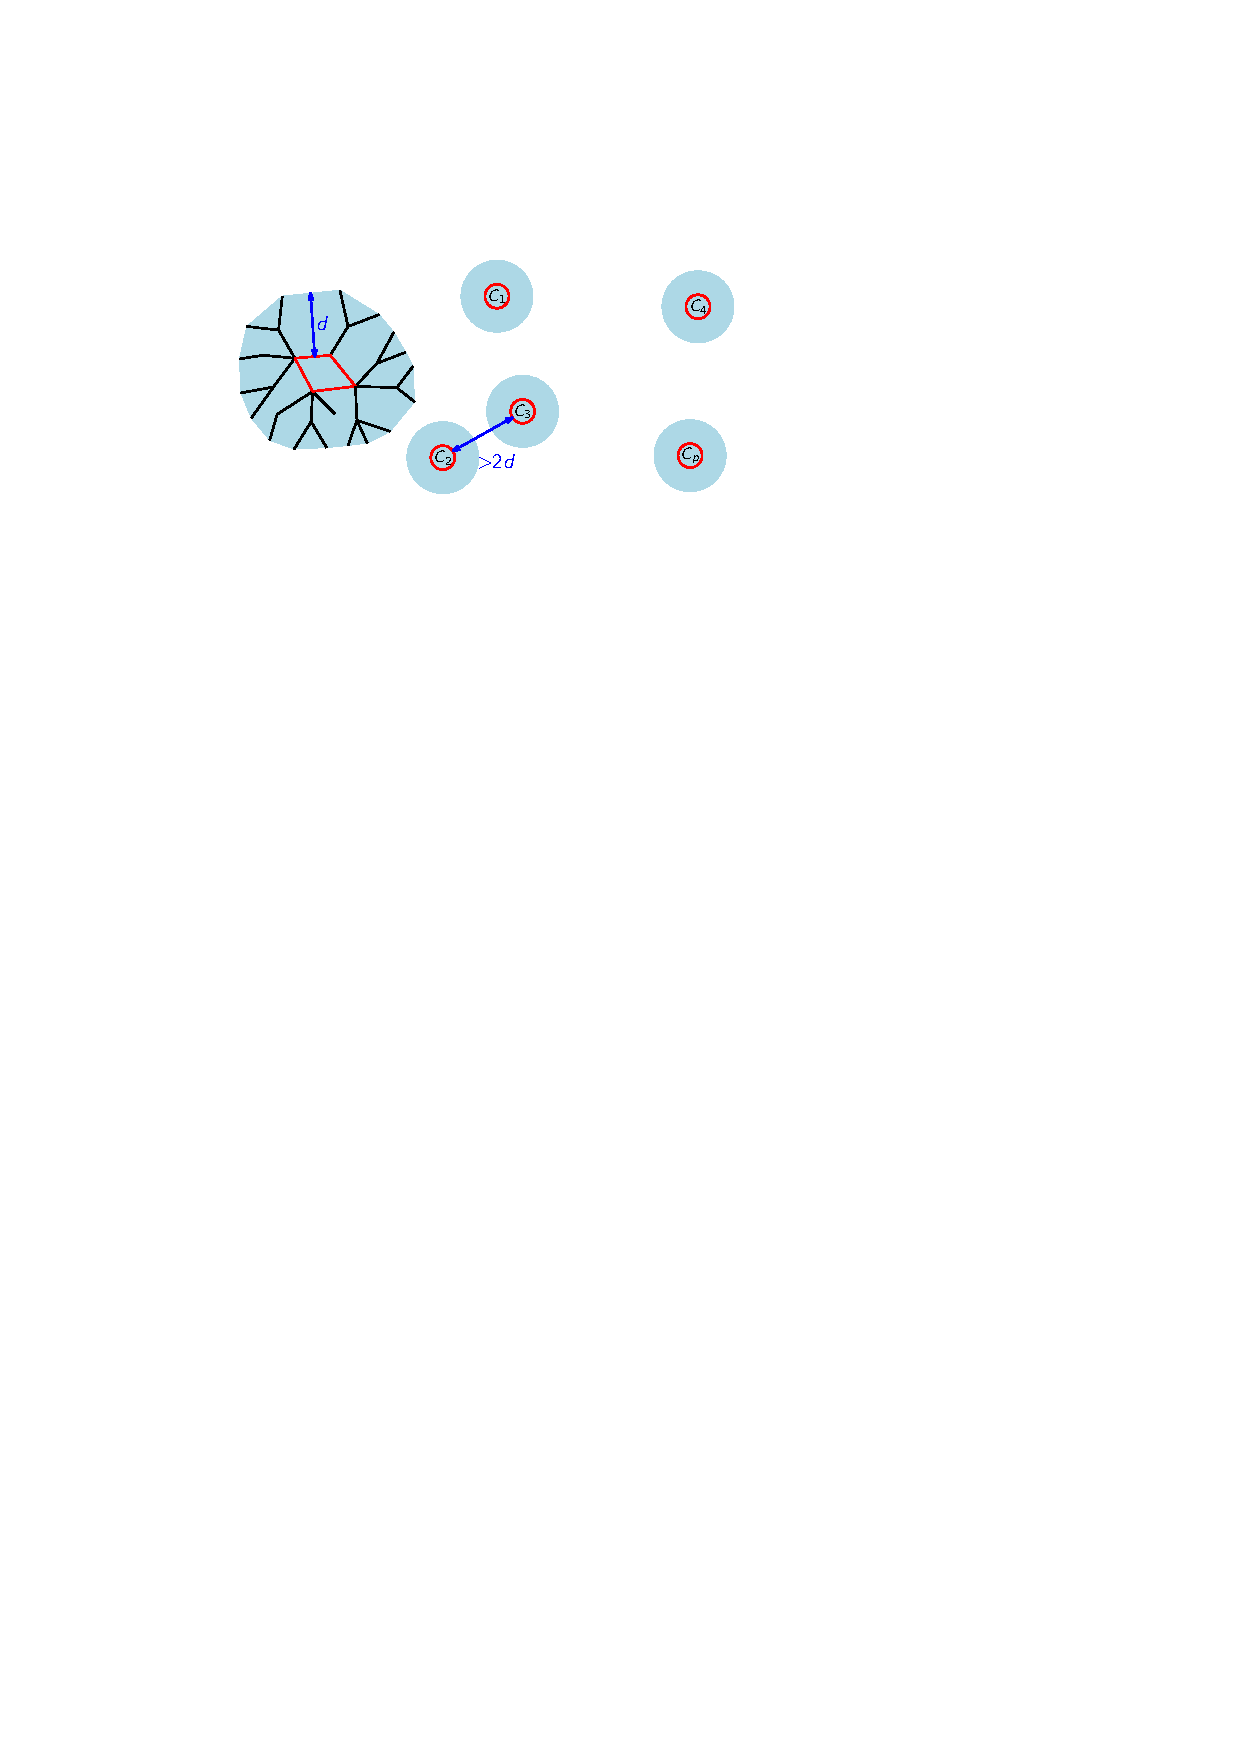
\includegraphics[page=1]{figs/animation}}%
  \only<2>{\includegraphics[page=2]{figs/animation}}%
  \only<3>{\includegraphics[page=3]{figs/animation}}%
  \only<4>{\includegraphics[page=4]{figs/animation}}%
  \only<5>{\includegraphics[page=5]{figs/animation}}%
  \only<6>{\includegraphics[page=6]{figs/animation}}%
  \only<7>{\includegraphics[page=7]{figs/animation}}%
  \only<8-9>{\includegraphics[page=8]{figs/animation}}%
  \only<10>{\includegraphics[page=9]{figs/animation}}%
  \only<11>{\includegraphics[page=10]{figs/animation}}%
  \only<12>{\includegraphics[page=11]{figs/animation}}%
  \only<13>{\includegraphics[page=12]{figs/animation}}%
  \only<14>{\includegraphics[page=13]{figs/animation}}%
  \only<15>{\includegraphics[page=14]{figs/animation}}%
  \only<16>{\includegraphics[page=15]{figs/animation}}%
  \only<17>{\includegraphics[page=16]{figs/animation}}%
  \only<18>{\includegraphics[page=17]{figs/animation}}%
  \only<19>{\includegraphics[page=18]{figs/animation}}%
  \only<20-21>{\includegraphics[page=19]{figs/animation}}%

  \begin{minipage}[t][5cm]{\textwidth}
    \only<1>{Start with maximal $2d$-packing $C_1,\ldots,C_p$ of $d$-unicyclic cycles\\ ($p < k$)}%
    \only<2>{\textbf{Lemma:} For any cycle $C$ in $G$:
    \begin{enumerate}
      \item[(i)] $C$ is \textcolor{blue}{close to} one of $C_1,\ldots,C_p$ or
      \item[(ii)] $C$ is \textcolor{blue}{close to} a \textcolor{blue}{short} cycle $C'$
    \end{enumerate}}%
    \only<3>{Iteratively hit each short cycle $C'$ with a single ball of radius $7d+1$}%
    \only<4>{Every (unhit) cycle in $G$ is \textcolor{blue}{close to} a cycle in $\mathcal{C}$}%
    \only<5-8>{\textbf{Lemma:} For each $i\in\{1,\ldots,p\}$,  $B(C_i,6d)-B(X_i,13d)$ is acyclic, for some $X_i$ with $|X_i|\le f'(k)$}%
    \only<9>{$F_i:=B(C_i,6d)-B(X_i,13d)$ is a forest, for each $i\in\{1,\ldots,p\}$}
    \only<10-12>{$F_0:=G-(\mathcolor{red}{B(X,7d+1)}\cup \mathcolor{blue}{\bigcup_{i=1}^p B(C_i,4d)})$ is a forest}%
    \only<13-14>{\textbf{Lemma:} For each distinct $i,j\in\{1,\ldots,p\}$, $B(C_i,6d)\cap B(C_j,6d)\subseteq B(X_{\{i,j\}},13d)$, for some $X_{\{i,j\}}$ with $|X_{\{i,j\}}|\le f'(k)$}
    \only<15>{$(\bigcup_{i=1}^p B(C_i,6d))-(\bigcup_i B(X_i,13d)\cup \bigcup_{i,j}(B(X_{\{i,j\}},13d))$ is a forest}
    \only<16-17>{Any remaining cycle contains a \textcolor{blue}{segment} with parts in $F_0$, $F_i$, and $F_j$\\
    Forget cycles and hit every segment}%
    \only<18>{Each segment $s$ has three parts $s_0$, $s_i$, $s_j$}%
    \only<19>{Extend $s_0$, $s_i$, and $s_j$}%
    \only<20>{$B(s_0,d)\subseteq F_0$, $B(s_i,d)\subseteq F_i$, and $B(s_j,d)\subseteq F_j$}%
    \only<21>{Map each segment to a $3$-subtree in the forest $F_0\uplus\biguplus_i F_i$}
  \end{minipage}
\end{frame}


\begin{frame}
  \frametitle{An Erdős-Pósa-Type Theorem for $c$-Subtrees}

  Recall:

  \noindent\textbf{Theorem (Gyárfás-Lehel 1970):} For every forest $F$, every integer $k'\ge 1$, and every collection $\mathcal{C}$ of $c$-subtrees of $F$,
  \begin{enumerate}%[nosep,nolistsep]
    \item[(a)] $\mathcal{C}$ contains $k'$ pairwise vertex-disjoint $c$-subtrees \textbf{or}
    \item[(b)] $G$ has a vertex subset $\mathcolor{red}{X}$ of size at most $\ell^\star(k',c)$ such that every $c$-subtree in $\mathcal{C}$ contains a vertex in $X$.
  \end{enumerate}
  \vspace{3ex}
  \uncover<2->{Apply this with $k'=Ck\log k$}\\[1ex]
  \uncover<3->{In Case~(b), $B(X,4d)$ hits every remaining cycle in $G$}
  \vspace{2ex}
\end{frame}

\begin{frame}
  \frametitle{Case~(a): $\mathcal{C}$ contains $k'$ pairwise vertex-disjoint $c$-subtrees}
  % In Case (a):\\
  \begin{center}
    \only<1>{\includegraphics[page=19,trim={1cm 2cm 2cm 0}]{figs/animation}}%
    \only<2>{\includegraphics[page=20,trim={1cm 2cm 2cm 0}]{figs/animation}}%
    \only<3->{\includegraphics[page=21,trim={1cm 2cm 2cm 0}]{figs/animation}}
  \end{center}
  \uncover<2->{Recall:\\
  \noindent\textbf{Theorem (Simonovits 1967):} Every (subdivision of every) cubic multigraph $G$ with at least $C k\log k$ vertices contains $k$ pairwise vertex-disjoint cycles.\hspace{2em} \uncover<3->{\Lightning}\uncover<4>{\hfill{QED}}
  }
\end{frame}

\begin{frame}
  \frametitle{Open Problems}

  \uncover<1->{Prove Main Theorem with $f(k)=O(k\log k)$ and $g(d)=c\cdot d$ \\[3ex]}
  \uncover<2->{
  \noindent\textbf{Conjecture (Georgakopoulos-Papasoglu 2023):} For every graph $G$
  \begin{enumerate}
    \item[(a)] $G$ has a $d$-fat $k\times K_3$ minor \textbf{or}
    \item[(b)] $G$ has a vertex subset $X$ of size at most $f(k)$ such that $G-B(X,g(k))$ has no $d$-fat $K_3$ minor.
  \end{enumerate}
  }
  \ \\[3ex]
  \uncover<3->{\Huge{\bf Thank You!}}
\end{frame}


\end{document}
